\documentclass[11pt,aspectratio=169]{beamer}

\usepackage[T1]{fontenc}
\usepackage{lmodern}
\usepackage{graphicx}
\usepackage{amsmath,amssymb,mathtools}
\usepackage{booktabs}
\usepackage{array}
\usepackage{multirow}
\usepackage{appendixnumberbeamer}

\setbeamercovered{transparent=5}
\setbeamertemplate{navigation symbols}{}
\setbeamertemplate{itemize items}[circle]
\setbeamertemplate{itemize subitem}{--}
\setbeamertemplate{footline}[frame number]
\setbeamerfont{framesubtitle}{size=\small}
\setbeamercolor{block title}{fg=black,bg=white!80!black}
\setbeamercolor{block body}{fg=black,bg=white!97!black}
\linespread{1.15}
\definecolor{citecolor}{RGB}{110,110,165}
\newcommand{\cit}[1]{{\color{citecolor}#1}}

\title{Fertility and Housing Tenure Choice:\\ Model and Population Closure}
\author{Tommaso De Santo}
\date{08/07/2026 \\[1ex] {\footnotesize Experimental repaired-E5 (floor) specification --- not the promoted benchmark}}

\begin{document}

{
\setbeamertemplate{footline}{}
\maketitle
}

% ---------------------------------------------------------------- roadmap
\begin{frame}{This Talk}
One-market national lifecycle model of housing and fertility. Since May:
\begin{itemize}
  \item \textbf{Fertility is sequential}: birth-by-birth attempts under declining fecundity, with children ever born and children at home tracked separately
  \item \textbf{Measured income risk}: after-tax persistent earnings process fixed outside the model
  \item \textbf{One housing market} (the two-location structure is set aside for the national question)
\end{itemize}
\vfill
Today's focus:
\begin{itemize}
  \item The \textbf{population closure}: what population-level statement can the model honestly make when fertility is endogenous and below replacement?
  \item Corrected \textbf{policy results} under the new closure
\end{itemize}
\end{frame}

\section{Model}

\begin{frame}[plain,c,noframenumbering]
\centering
{\Large\textbf{Model}}
\end{frame}

% ---------------------------------------------------------------- environment
\begin{frame}{Environment}
\small
\begin{itemize}\setlength\itemsep{2pt}
  \item \textbf{Agents.} A mass $S$ of households; age $j=1,\dots,17$ four-year periods from age 18; retirement at 65; survival risk in old age
  \item \textbf{Children.} Two state variables per household: $n$ children ever born, $m$ children currently at home; each child at home matures independently with per-period probability $2/9$ (18 expected years at home); two matured children form one new potential household
  \item \textbf{Endowments.} Entrants start as childless renters on a fixed entry-wealth distribution; persistent after-tax earnings risk (next slide); exogenous wage level and interest rate
  \item \textbf{Markets.} One housing market: rental services and owned houses (ladder); one-period bond; no aggregate risk
  \item \textbf{Institutions.} Property tax $\tau_H$ with a balanced-budget lump-sum transfer; payroll tax and stationary pension; warm-glow bequests --- estates are valued by parents but transfer to no one
  \item \textbf{Entry.} New households enter at age 18: retained matured city-born children plus an outside inflow (the closure; Section 3)
\end{itemize}
\end{frame}

% ---------------------------------------------------------------- preferences
\begin{frame}{Preferences}
Flow utility over consumption and housing services, scaled by family size:
\[
u(c,\mathbf h; m)
= \frac{\Big[\big(c/e_c(m)\big)^{\alpha}\big(\mathbf h/e_h(m)\big)^{1-\alpha}\Big]^{1-\sigma}}{1-\sigma}
+ \psi_{\mathrm{child}}\, m ,
\qquad \sigma = 2,
\]
with equivalence scales $e_c(m), e_h(m)$ increasing in children at home.
\begin{itemize}
  \item \textbf{Owner premium.} Housing services are $\chi h$ for owners ($\chi>1$) and $h^R$ for renters
  \item \textbf{Child space floor} (this arm): each child at home requires $\underline h$ rooms --- the estimated floor is $0.61$ rooms per child
  \item \textbf{Bequests.} Warm glow at death over terminal wealth $b + p h$, curvature shifted by $(\theta_0,\theta_1)$
\end{itemize}
\smallskip
The estimated child flow utility $\psi_{\mathrm{child}}$ is zero at this winner: children are valued through the choice structure, not a flow term.
\end{frame}

% ---------------------------------------------------------------- fertility
\begin{frame}{Sequential Fertility}
Births arrive one at a time through an attempt margin under biological limits:
\begin{itemize}
  \item In the fecund window, a household chooses each period whether to \textbf{attempt} a birth: a discrete choice with taste shocks (scale $\kappa_f$ for the first birth, $\kappa_f^{\mathrm{cont}}$ for subsequent births)
  \item An attempt succeeds with an age-declining \textbf{fecundity} probability --- timing is chosen, arrival is risky
  \item A birth moves the household $(n,m)\to(n+1,m+1)$; children at home raise the equivalence scales and the room floor, then mature out
\end{itemize}
\medskip
The margin this delivers: households postpone attempts when housing is expensive and run into the fecundity clock --- the mechanism connecting housing costs to completed fertility and childlessness.
\end{frame}

% ---------------------------------------------------------------- income
\begin{frame}{Earnings and Institutions}
After-tax earnings are fixed outside the model from measured objects:
\[
\log y_{j+1} = \rho \log y_j + \varepsilon, \qquad
\rho = 0.914, \quad \sigma_\varepsilon^{\mathrm{annual}} = 0.169,
\]
a five-state Rouwenhorst discretization, aggregated to four-year periods.
\begin{itemize}
  \item Persistence and innovation variance from the panel literature; progressivity retention $1-\tau = 0.819$ (HSV, $\tau=0.181$)
  \item Age profile of earnings; payroll tax $0.179$ funds a stationary pension
  \item Property tax $\tau_H$ (baseline 1\% annual) rebated lump-sum --- the policy instrument later
\end{itemize}
\smallskip
Income risk is measurement, not calibration: no earnings parameter is estimated.
\end{frame}

% ---------------------------------------------------------------- housing
\begin{frame}{Housing, Tenure, and Budget Sets}
A household either rents or owns:
\[
h^R \in (0, \bar h^R], \qquad h \in \{H_1,\dots,H_6\} = \{2,\dots,11\} \text{ rooms},
\qquad \bar h^R = 6.
\]
\textbf{Renters} pay rent $r h^R$, save $b'\ge 0$. \quad \textbf{Owners} post a down payment and borrow against the house:
\[
b' \;\ge\; -\phi\, p h, \qquad \phi = 0.80 \;\;(\text{20\% down}),
\]
pay maintenance $\delta$, property tax $\tau_H$, and a transaction cost $\psi$ when adjusting.
\begin{itemize}
  \item \textbf{Segmentation:} the largest rental is smaller than the largest owned unit, so family-sized space is reached through ownership --- the down payment is the barrier a birth must clear
\end{itemize}
\end{frame}

% ---------------------------------------------------------------- supply/equilibrium
\begin{frame}{Housing Supply and Equilibrium}
Supply is an upward-sloping curve in \textbf{levels}, and rents are tied to prices by user cost:
\[
H^S = H_0\left(\frac{r}{\bar r}\right)^{\xi},
\qquad
r = (q+\delta+\tau_H)\,p .
\]
\begin{itemize}
  \item One market-clearing condition: aggregate services demanded $=$ $H^S$
  \item The level curve is the fixed-land statement: a permanently larger population permanently raises rents --- this is what makes the population question bite
  \item Stationary equilibrium: prices, the transfer, and the household distribution constant; the government budget clears
\end{itemize}
\smallskip
Wages and the interest rate stay exogenous: the housing market is the only price feedback.
\end{frame}

% ---------------------------------------------------------------- household problem
\begin{frame}{The Household's Problem}
Within a period: attempt decision, then tenure, housing, and saving:
\[
V_j(b,h,y,n,m)
= \mathbb{E}_{\varepsilon}\max_{a\in\{0,1\}}
\Big\{ \underbrace{W_j^{a}(b,h,y,n,m)}_{\text{tenure/housing/saving problem}} + \varepsilon_a \Big\},
\]
where an attempt ($a=1$) succeeds with fecundity $\pi_j$ and, if successful, delivers $(n+1,m+1)$ next period. The inner problem chooses rent-vs-own, the housing quantity or rung, consumption, and $b'$ subject to the budget and collateral constraints, with deterministic tenure choice.
\medskip

Old age: no attempts, survival risk, warm-glow bequest at death; matured children leave the state vector and join the entrant pool.
\end{frame}

\section{Calibration}

\begin{frame}[plain,c,noframenumbering]
\centering
{\Large\textbf{Calibration}}
\end{frame}

% ---------------------------------------------------------------- external
\begin{frame}{Externally Fixed Objects}
\small
\centering
\renewcommand{\arraystretch}{0.95}
\begin{tabular}{llcl}
\toprule
& \textbf{Object} & \textbf{Value} & \textbf{Source} \\
\midrule
\textit{Pref.} & $\sigma$ risk aversion & 2.0 & standard \\
\textit{Fin.} & $q$ interest (annual) & 0.04 & standard \\
& $\delta$ depreciation (annual) & 0.02 & Greaney et al. \\
& $\tau_H$ property tax (annual) & 0.01 & US average \\
& $\phi$ financed share & 0.80 & 20\% down payment \\
& $\psi$ transaction cost & 0.06 & Greaney et al. \\
\textit{Life} & 17 four-year periods & ages 18--85 & retirement 65 \\
\textit{Income} & $\rho$, $\sigma_\varepsilon$, HSV $\tau$ & $0.914$, $0.169$, $0.181$ & FL $\times$ HSV \\
& $\tau_{\mathrm{pay}}$ payroll & 0.179 & Greaney et al. \\
\textit{Children} & maturation hazard & $2/9$ per period & 18 expected years \\
\textit{Housing} & ladder, rental cap & $\{2,\dots,11\}$, $6$ rooms & room units \\
\bottomrule
\end{tabular}

\medskip
\raggedright
External restriction on the search: annual $\beta \ge 0.94$.
\end{frame}

% ---------------------------------------------------------------- internal
\begin{frame}{Estimated Parameters (floor arm)}
\small
\centering
\renewcommand{\arraystretch}{0.92}
\begin{tabular}{llccc}
\toprule
\textbf{Param} & \textbf{Description} & \textbf{Estimate} & \textbf{Bounds} & \textbf{Near bound?} \\
\midrule
$\beta$ (annual) & Discount factor & 0.9946 & $[0.94, 0.9995]$ & no \\
$\psi_{\mathrm{child}}$ & Child flow utility & 0.000 & $[0,3]$ & \textbf{at lower} \\
$\kappa_f$ & Attempt taste scale, first birth & 2.987 & $[0.02,50]$ & no \\
$\kappa_f^{\mathrm{cont}}$ & Attempt taste scale, later births & 1.713 & $[0.02,50]$ & no \\
$\chi$ & Owner service premium & 1.037 & $[0.1,5]$ & no \\
$H_0$ & Housing supply intercept & 9.873 & $[0.2,80]$ & no \\
$\theta_0$ & Bequest strength & 0.159 & $[0,8]$ & \textbf{near lower} \\
$\theta_1$ & Bequest shifter & 0.094 & $[0.02,16]$ & \textbf{near lower} \\
$\underline h$ & Child room floor & 0.614 & $[0.1,1.8]$ & no \\
\bottomrule
\end{tabular}

\medskip
\raggedright
Nine free parameters against twelve moments. The bequest block sits near its lower bounds and the child flow utility is exactly zero: saving-for-bequests and direct child utility are doing little work at this winner.
\end{frame}

% ---------------------------------------------------------------- fit
\begin{frame}{Target Fit (floor arm; loss 297.1)}
\centering
\fontsize{7.4}{8.8}\selectfont
\setlength{\tabcolsep}{3.5pt}
\renewcommand{\arraystretch}{0.85}
\begin{tabular}{@{}llrrrr@{}}
\toprule
& \textbf{Moment} & \textbf{Target} & \textbf{Model} & \textbf{Gap} & \textbf{Contr.} \\
\midrule
\textit{Fertility} & Completed fertility & 1.918 & 1.967 & $+0.049$ & 3.4 \\
& Childlessness & 0.188 & 0.104 & $-0.084$ & \textbf{121.5} \\
& Mean age at first birth & 25.31 & 25.57 & $+0.26$ & 1.1 \\
& First births at 30+ & 0.270 & 0.327 & $+0.057$ & \textbf{51.5} \\
\midrule
\textit{Housing} & Rooms response to first birth & 0.664 & 0.690 & $+0.026$ & 0.6 \\
& Rooms, 3+ vs.\ 1--2 children & 0.368 & 0.359 & $-0.009$ & 0.2 \\
& Family ownership gap & 0.168 & 0.162 & $-0.006$ & 0.5 \\
& Ownership rate & 0.575 & 0.582 & $+0.007$ & 0.1 \\
& Aggregate mean rooms & 5.780 & 6.478 & $+0.698$ & 5.8 \\
\midrule
\textit{Wealth} & Wealth / earnings & 6.873 & 5.794 & $-1.079$ & 7.3 \\
& Bequest flow / wealth & 0.0088 & 0.0087 & $-0.0001$ & 0.0 \\
& Old wealth p90/p50 & 3.448 & 2.090 & $-1.358$ & \textbf{105.1} \\
\bottomrule
\end{tabular}

\medskip
\raggedright\small
Three rows carry 94\% of the loss: childlessness, old-age wealth dispersion, late first births. An overnight 16-chain multi-start on the unchanged contract (fresh seeds; 24 chains total) finds nothing better: these are \textbf{mechanism limits, not search failures}.
\end{frame}

% ---------------------------------------------------------------- fit figures
\begin{frame}{Lifecycle Fit}
\centering

\includegraphics[width=0.49\textwidth,height=0.78\textheight,keepaspectratio]{../output/model/eqscale_seq_e5_policy_quota_closure_20260807/diagnostics/floor/standard/fertility_by_age.png}\hfill

\includegraphics[width=0.49\textwidth,height=0.78\textheight,keepaspectratio]{../output/model/eqscale_seq_e5_policy_quota_closure_20260807/diagnostics/floor/standard/ownership_by_age.png}

\smallskip
{\footnotesize Standard diagnostic packet; full set in the appendix and in the packet folder.}
\end{frame}

\section{Population Closure}

\begin{frame}[plain,c,noframenumbering]
\centering
{\Large\textbf{Population Closure}}
\end{frame}

% ---------------------------------------------------------------- closure problem
\begin{frame}{The Closure Problem}
With endogenous below-replacement fertility, a closed stationary population cannot exist:
\[
\underbrace{B_0 \approx 0.053}_{\text{matured city-born flow}}
\;<\;
\underbrace{E_0 \approx 0.062}_{\text{entrants needed for stationarity}}
\qquad\Rightarrow\qquad
\text{natives replace } \sim\!86\% \text{ of each cohort.}
\]
Some outside inflow must close the gap --- exactly the U.S.\ situation, where net international migration now accounts for most population growth.
\medskip

\textbf{The previous device:} entrants compared value inside to an outside value $\bar V^{out}$ and entered with logit probability ($\lambda=2$). Three problems:
\begin{enumerate}
  \item $\lambda$ is unidentified --- and generated $\sim 90\%$ of the $+9$--$10\%$ policy population responses
  \item The margin is nearly saturated ($q^*=0.97$): responses are one-sided by construction
  \item Holding the outside fixed while a \emph{national} policy moves all inside values is a single-treated-city experiment in a one-market national model
\end{enumerate}
\end{frame}

% ---------------------------------------------------------------- quota closure
\begin{frame}{The Quota Closure}
Delete the choice layer; hold the flows themselves fixed:
\[
S\,E_0 \;=\; \bar R\, S\, B_0(\text{policy}) \;+\; \bar M,
\qquad
\bar R = \frac{(1-s^{out})E_0}{B_0} = 0.969,
\quad
\bar M = s^{out} E_0,
\]
with $s^{out}=0.169$ the outside-origin share of entrants. Institutions justify the invariance: U.S.\ immigration is quantity-rationed and oversubscribed --- the marginal entrant is set by the quota, not by indifference.
\begin{itemize}
  \item Baseline is \textbf{bit-identical} to the old one (the logit was reverse-engineered to this same accounting); zero recalibration
  \item Population responds through the one margin the model disciplines --- births --- with renewal multiplier $(1-s^{out})/s^{out} = 4.92$, damped by housing scarcity
  \item Below-replacement fertility $+$ a constant absolute inflow $\Rightarrow$ a stationary population exists and is stable (standard demography)
\end{itemize}
\end{frame}

\section{Policy}

\begin{frame}[plain,c,noframenumbering]
\centering
{\Large\textbf{Policy Results}}
\end{frame}

% ---------------------------------------------------------------- policy results
\begin{frame}{Funded Property-Tax and Grant Reforms}
Raise the property tax from 1\% to 2\%; rebate lump-sum, or fund a purchase grant for family-sized homes. All changes vs.\ the funded 1\% baseline, percent:
\medskip

\centering
\small
\renewcommand{\arraystretch}{0.95}
\begin{tabular}{llrrrrrr}
\toprule
Arm & Policy & TFR & Births & Househ. & $-\Delta$Imm. & Price & Rent \\
\midrule
Floor & 2\% tax          & $+0.38$ & $+0.33$ & $+1.70$ & $1.74$ & $-17.5$ & $-6.1$ \\
Floor & tax + grant      & $+0.75$ & $+0.67$ & $+3.46$ & $3.52$ & $-17.3$ & $-5.8$ \\
Tilt  & 2\% tax          & $+0.20$ & $+0.18$ & $+0.90$ & $0.92$ & $-17.7$ & $-6.3$ \\
Tilt  & tax + grant      & $+0.49$ & $+0.44$ & $+2.23$ & $2.26$ & $-17.2$ & $-5.7$ \\
\bottomrule
\end{tabular}

\medskip
\raggedright
\small
In U.S.\ units: $+0.33$--$0.67\%$ births is roughly $12$--$24$ thousand extra babies per year immediately; the household-count response ($+1.7$--$3.5\%$) is the stationary limit, reached on a $\sim$century timescale. The price falls because the tax lowers owner demand --- the \textbf{down-payment barrier} drops $17.5\%$ while renter rent (tax-inclusive) falls only $6\%$.
\end{frame}

% ---------------------------------------------------------------- interpretation
\begin{frame}{What the Population Numbers Mean}
One number, three equivalent units --- all renewal arithmetic on the birth response:
\begin{center}\small
households $+3.5\%$ \;$\Longleftrightarrow$\; required immigration $-3.5\%$ at fixed population\\[2pt]
$\Longleftrightarrow$\; $3.5\%$ of the fertility gap closed.
\end{center}
\begin{itemize}
  \item \textbf{Housing feedback is real but small}: the arithmetic multiplier overstates the realized response by only $0.02$--$0.10$pp --- scarcity makes pronatal policy mildly self-limiting
  \item \textbf{Honest headline change}: $+0.9$--$3.5\%$, not the withdrawn $+9$--$10\%$ (that was $\lambda$)
  \item \textbf{Timing}: half the gap closes in $\sim$a century; the immediate objects are the birth and required-immigration flows
\end{itemize}
\end{frame}

% ---------------------------------------------------------------- open items
\begin{frame}{Open Decisions}
\begin{enumerate}
  \item \textbf{The anchor concept.} New ACS measurement: recent immigrants are only $3.7\%$ of age-18--22 household entrants --- below the $14.3\%$ feasibility floor. But immigrants mostly arrive \emph{older} than the stylized entry age. Recommended: anchor $\bar M$ to \emph{age-aggregated} net migration ($\sim 0.17$--$0.22$, brackets the provisional $0.169$); the alternative is multi-age immigrant entry
  \item \textbf{The fertility block.} Closure feasibility requires $B_0/E_0 \ge 0.831$; the repaired-E5 chain-6 winner fails it (screened out), and the misses that survive 24 chains --- childlessness, old-age wealth dispersion, late first births --- are mechanism questions, not calibration slack
  \item \textbf{Scope.} Welfare comparisons stay per-household; the entry margin, if it ever needs to be behavioral, is household formation (headship), not an international logit
\end{enumerate}
\vfill
\centering
\textit{Population effects are now: births $\times$ transparent demography, damped by housing scarcity --- conditional on fixed immigration.}
\end{frame}

\appendix

\begin{frame}[plain,c,noframenumbering]
\centering
{\Large\textbf{Appendix}}
\end{frame}

\begin{frame}{Appendix: Housing Market Diagnostics}
\centering

\includegraphics[width=0.49\textwidth,height=0.78\textheight,keepaspectratio]{../output/model/eqscale_seq_e5_policy_quota_closure_20260807/diagnostics/floor/standard/housing_market.png}\hfill

\includegraphics[width=0.49\textwidth,height=0.78\textheight,keepaspectratio]{../output/model/eqscale_seq_e5_policy_quota_closure_20260807/diagnostics/floor/standard/owner_rungs.png}
\end{frame}

\begin{frame}{Appendix: Wealth and Tenure Diagnostics}
\centering

\includegraphics[width=0.49\textwidth,height=0.78\textheight,keepaspectratio]{../output/model/eqscale_seq_e5_policy_quota_closure_20260807/diagnostics/floor/standard/liquid_wealth_by_age_income_state.png}\hfill

\includegraphics[width=0.49\textwidth,height=0.78\textheight,keepaspectratio]{../output/model/eqscale_seq_e5_policy_quota_closure_20260807/diagnostics/floor/standard/tenure_services.png}
\end{frame}

\begin{frame}{Appendix: Policy Comparison}
\centering
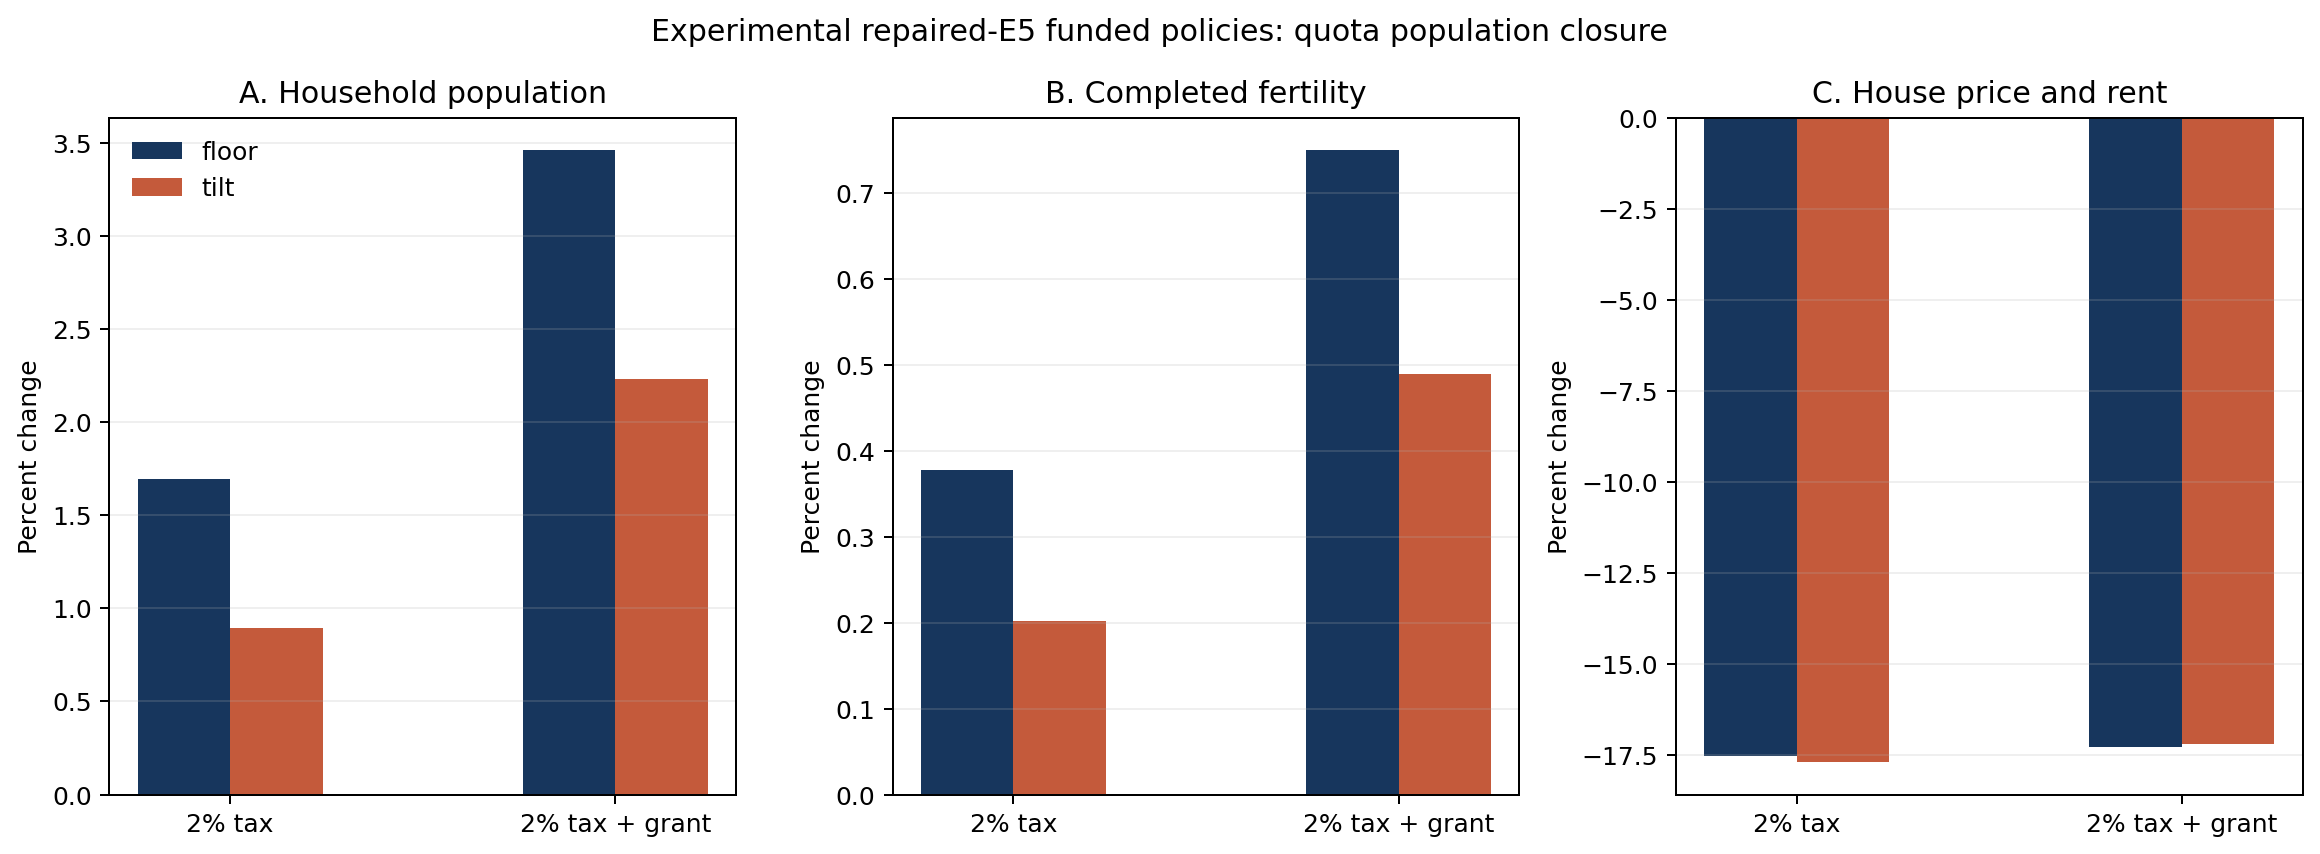
\includegraphics[width=0.9\textwidth,height=0.82\textheight,keepaspectratio]{../output/model/eqscale_seq_e5_policy_quota_closure_20260807/diagnostics/policy/quota_policy_comparison.png}
\end{frame}

\begin{frame}{Appendix: Anchor Sensitivity and Convergence Speed}
\centering
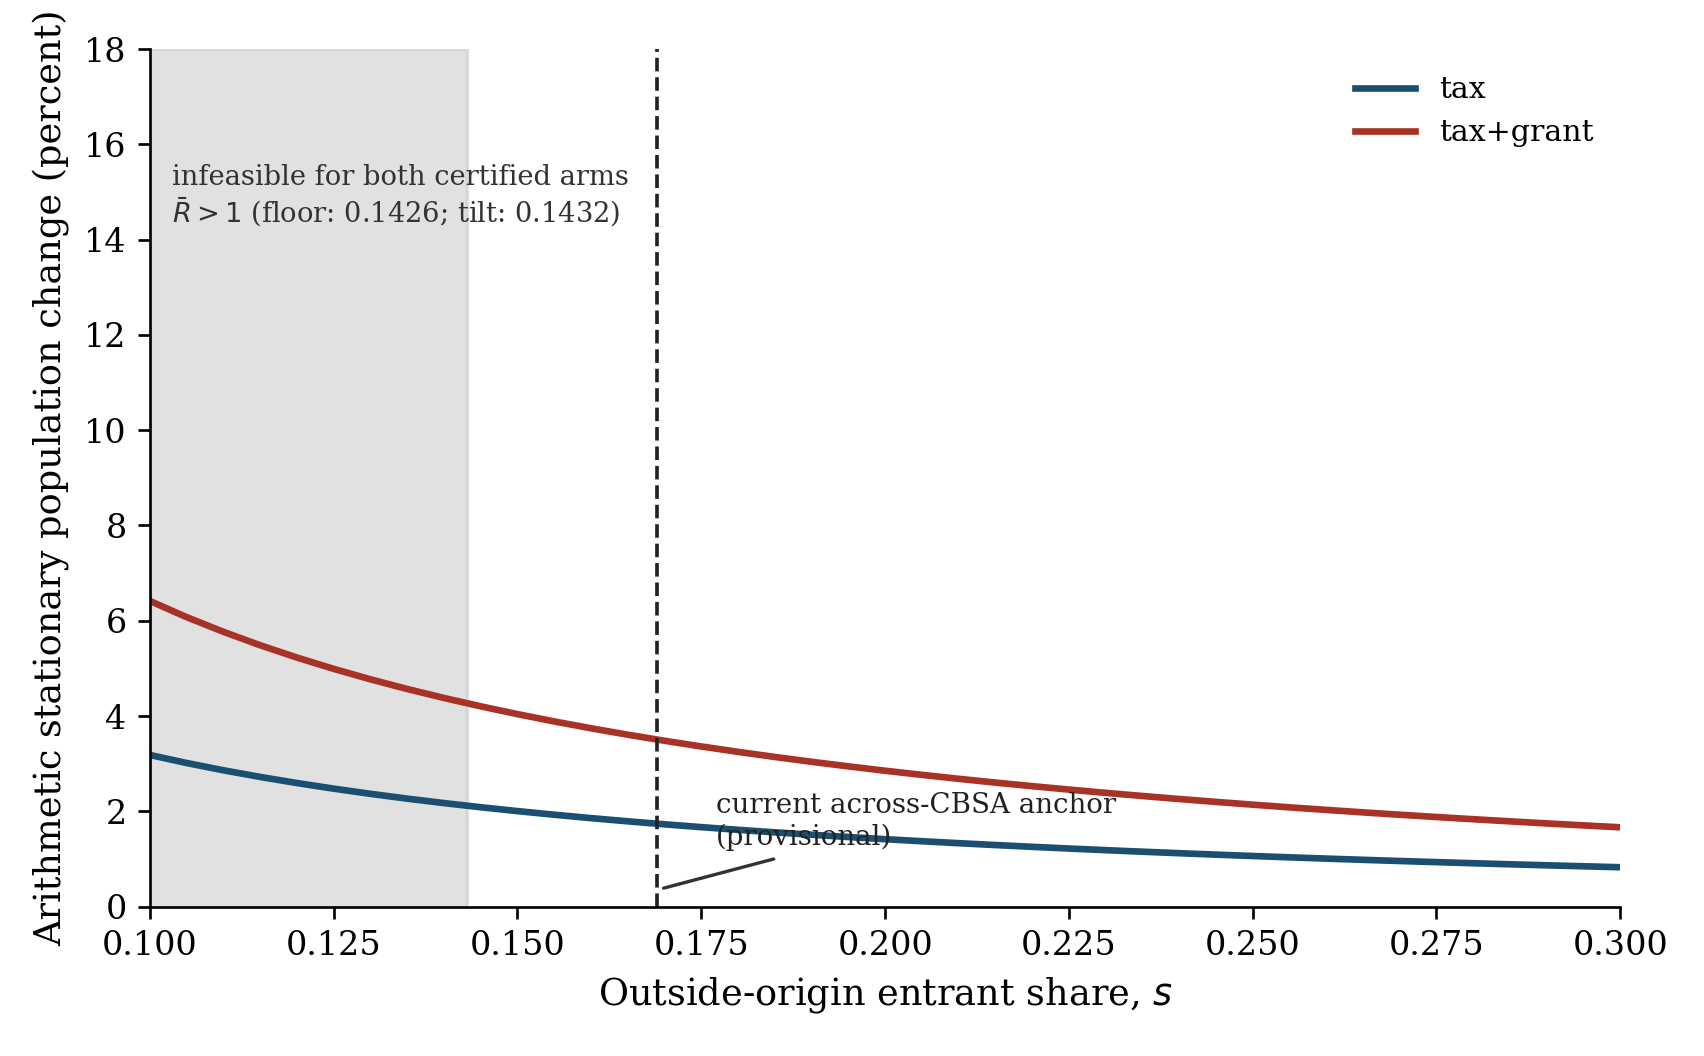
\includegraphics[width=0.62\textwidth,height=0.62\textheight,keepaspectratio]{../output/model/population_closure_arithmetic_20260807/anchor_sensitivity.png}

\smallskip
\raggedright\footnotesize
Stationary population response as a function of the outside-origin share $s^{out}$, with the infeasible region ($s^{out}<0.143$) shaded. Convergence: generational decay $\rho = \bar R B_0/E_0 = 0.831$ gives a half-life of $97$--$112$ years ($g=26$--$30$); an age-structured variant with uniform birth timing gives $\sim 230$ years (upper bound).
\end{frame}

\begin{frame}{Appendix: The Retired Logit as a Sensitivity Row}
\footnotesize
The old protocol's numbers survive as a labeled robustness row, not a model:
\medskip

\centering
\begin{tabular}{llrr}
\toprule
Arm & Policy & Quota population & Logit sensitivity ($\lambda=2$, unidentified) \\
\midrule
Floor & 2\% tax     & $+1.70$ & $+9.98$ \\
Floor & tax + grant & $+3.46$ & $+10.10$ \\
Tilt  & 2\% tax     & $+0.90$ & $+8.99$ \\
Tilt  & tax + grant & $+2.23$ & $+9.06$ \\
\bottomrule
\end{tabular}

\medskip
\raggedright
The gap between columns is what an unidentified taste parameter was contributing. The logit row bounds ``what if entry responded to values'' without pretending to identify it.
\end{frame}

\begin{frame}{Appendix: National Entry-Anchor Measurement (ACS 2012--2023)}
\footnotesize
\centering
\begin{tabular}{lrr}
\toprule
Measure (household heads unless noted) & Share & Multiplier $(1-s)/s$ \\
\midrule
Ages 18--22, foreign-born, arrived $\le 4$y (headline) & 3.71\% & 25.9 \\
Ages 18--22, foreign-born, arrived $\le 8$y & 5.36\% & 17.7 \\
Ages 18--25, foreign-born, arrived $\le 4$y & 3.47\% & 27.9 \\
Ages 18--22, foreign-born stock (upper bound) & 9.04\% & 10.1 \\
Persons 18--22, foreign-born, arrived $\le 4$y & 2.89\% & 33.7 \\
\midrule
Quota feasibility floor & 14.3\% & --- \\
Age-aggregated net-migration bracket (to verify) & 17--22\% & 3.5--4.9 \\
\bottomrule
\end{tabular}

\medskip
\raggedright
Every entry-age-window measure is infeasible; the age-aggregated concept is not. The two are different objects because immigrants mostly arrive above the stylized entry age --- the anchor decision on the Open Decisions slide.
\end{frame}

\begin{frame}{Appendix: Multi-Start Record (overnight)}
\footnotesize
16 fresh chains, unchanged 12-moment / 9-parameter contract, 225-minute budget each, strict-repeat certification:
\medskip

\centering
\begin{tabular}{lrrr}
\toprule
& Best & Median & Worst \\
\midrule
Fresh chains (seeds 09--24) & 263.5 & $\sim$284 & 370.5 \\
Certified incumbent (Aug 5, chain 6) & \multicolumn{3}{c}{249.186 --- \textbf{stands}} \\
\bottomrule
\end{tabular}

\medskip
\raggedright
All 16 eligible with exact strict repeats on the run's best; market residuals $\le 2.2\times 10^{-5}$. With 24 chains total across the two arrays, the remaining misses are search-converged.
\end{frame}

\end{document}
